\documentclass[11pt,a4paper,fontset=fandol]{ctexart}

% ---------- 宏包 ----------
\usepackage[a4paper,margin=2.3cm]{geometry}
\usepackage{amsmath}
\usepackage{amssymb}
\usepackage{graphicx}
\usepackage{xcolor}
\usepackage{booktabs}
\usepackage{tabularx}
\usepackage{array}
\usepackage{longtable}
\usepackage{enumitem}
\usepackage{listings}
\usepackage{tikz}
\usepackage{caption}
\usepackage{titlesec}
\usepackage{microtype}
\usepackage{hyperref}
\usetikzlibrary{shapes.geometric,arrows.meta,positioning,fit,backgrounds,calc}

% ---------- 颜色 ----------
\definecolor{primary}{RGB}{18,158,120}
\definecolor{accent}{RGB}{74,124,255}
\definecolor{ink}{RGB}{30,38,52}
\definecolor{soft}{RGB}{120,135,158}
\definecolor{codebg}{RGB}{246,248,251}
\definecolor{codecmt}{RGB}{60,140,90}
\definecolor{codekw}{RGB}{40,90,200}
\definecolor{codestr}{RGB}{170,80,40}

\hypersetup{colorlinks=true,linkcolor=primary,urlcolor=accent,citecolor=primary,
  pdftitle={Anker AI 原生产品定义系统 技术报告},pdfauthor={戴尚好}}

% ---------- 标题格式 ----------
\titleformat{\section}[block]
  {\Large\bfseries\color{primary}}{\thesection}{0.6em}{}
  [\vspace{-0.4em}{\color{primary}\rule{\linewidth}{1.0pt}}]
\titleformat{\subsection}[block]
  {\large\bfseries\color{ink}}{\thesubsection}{0.5em}{}

% ---------- 代码风格 ----------
\lstset{
  basicstyle=\scriptsize\ttfamily,
  backgroundcolor=\color{codebg},
  breaklines=true,
  breakatwhitespace=false,
  columns=fullflexible,
  keepspaces=true,
  showstringspaces=false,
  frame=single,
  rulecolor=\color{soft!40},
  commentstyle=\color{codecmt},
  keywordstyle=\color{codekw}\bfseries,
  stringstyle=\color{codestr},
  numbers=left,
  numberstyle=\tiny\color{soft},
  numbersep=6pt,
  tabsize=4,
  xleftmargin=1.6em,
}

\newcommand{\kw}[1]{\textbf{\color{primary}#1}}
\setlist{nosep,leftmargin=1.4em}

% ====================================================================
\begin{document}

% ---------------- 封面 ----------------
\begin{titlepage}
\centering
\vspace*{2.2cm}
{\fontsize{16}{20}\selectfont\color{soft} 2026 AI 先锋未来人才大赛 · 安克创新命题 · 华南赛区}\\[0.4cm]
{\color{soft}\rule{0.5\linewidth}{0.4pt}}\\[1.4cm]
{\fontsize{34}{42}\selectfont\bfseries\color{primary} Anker AI 原生\\[0.2cm]产品定义系统}\\[1.0cm]
{\fontsize{15}{22}\selectfont\color{ink} 让 AI 做你的\textbf{超级智囊 · 用户替身 · 行业专家}}\\[0.3cm]
{\fontsize{13}{20}\selectfont\color{soft} 从真实用户数据，到一份可溯源、可验证、可量化的产品提案}\\[2.2cm]

\begin{tikzpicture}
  \node[draw=primary,rounded corners=8pt,line width=1pt,inner sep=10pt,text width=12cm,align=center,text=ink]
  {\small 一套真实可运行的多智能体系统：把安克 JML / BEES / AMI 三大产品方法论平台做成 AI 原生版，
   端到端从真实评论跑出产品提案，并用受控实验回答——\textbf{AI 驱动相较"经验拍脑袋"的本质不同}。};
\end{tikzpicture}

\vfill
{\large\bfseries 戴尚好}\\[0.2cm]
{\color{soft} 中国科学技术大学}\\[0.2cm]
{\color{soft} 2026 年 6 月}
\end{titlepage}

% ---------------- 作者 / 链接页 ----------------
\thispagestyle{empty}
\vspace*{1.2cm}
\section*{参赛信息与项目链接}
\vspace{0.4cm}
{\renewcommand{\arraystretch}{1.4}
\begin{tabularx}{\linewidth}{p{3.2cm} X}
\toprule
\textbf{参赛者} & 戴尚好 \\
\textbf{学校} & 中国科学技术大学 \\
\textbf{赛道 / 命题} & AI + 研发创新 ；安克创新——用 AI 重做一次产品设计与定义 \\
\textbf{赛区} & 华南 \\
\textbf{邮箱} & \href{mailto:bcefghj@163.com}{bcefghj@163.com} \\
\textbf{个人主页} & \url{https://bcefghj.github.io} \\
\textbf{GitHub 源码} & \url{https://github.com/bcefghj/anker-ai-product-studio} \\
\textbf{在线 Demo} & \url{http://47.119.112.225/anker/app/} \\
\textbf{项目宣传页} & \url{http://47.119.112.225/anker/} \\
\textbf{项目导航 Hub} & \url{http://47.119.112.225/} \\
\bottomrule
\end{tabularx}}

\vspace{0.8cm}
\noindent\textbf{\color{primary}一句话摘要。}\;
本作品不是 PPT，而是一套真实可运行、数据可溯源、可评测的多智能体系统。它把安克内部真实的产品方法论平台
JML/BEES/AMI 做成 AI 原生版，让 AI 扮演超级智囊、用户替身、行业专家，端到端从真实用户评论跑出一份产品提案
（Working Backwards PR/FAQ），并用一个受控对比实验量化回答命题：在同一 brief 下，AI 原生工作流相较"经验拍脑袋"，
命中真实痛点率由 33\% 提升到 100\%、可溯源证据引用由 0 增至 56 条、预测 NPS 提升约 30 分。系统遵循对标大厂的
AIGC 工程规范（四层架构、AI Rule、Pre-PR、跨厂商模型对抗 CR），并已部署上线（与既有项目按目录/端口/路由隔离，互不影响）。

\newpage
\tableofcontents
\newpage

% ====================================================================
\part{命题理解与背景洞察}
\section{大赛与命题}

2026 AI 先锋未来人才大赛由飞书与数智教育发展国际大学联盟主办、教育部指导。安克创新（深交所 300866）
给出的命题是：

\begin{quote}\itshape
假设你要为安克设计一款创新产品，让 AI 做你的超级智囊、用户替身、行业专家——用这种新方法从头做一次产品设计与定义，
比比看和靠经验拍脑袋有什么本质不同？
\end{quote}

交付物有两层：(1) 选一个安克品类，设计并演示一套"AI 原生"的产品设计与定义工作流，产出一份产品提案
（用户洞察 + 产品概念 + 可行性分析）；(2) 说明这个 AI 原生方法论，并与传统方法对比（AI 驱动 vs 经验驱动，差异是什么）。

\section{安克是谁：用数据说话}

\begin{table}[h]\centering\small
\renewcommand{\arraystretch}{1.25}
\begin{tabularx}{\linewidth}{p{4.6cm} X}
\toprule
\textbf{指标（2025 年报）} & \textbf{数据} \\
\midrule
营收 & 305.14 亿元（首破 300 亿，同比 +23.49\%） \\
归母净利润 & 25.45 亿元（同比 +20.37\%） \\
研发投入 & 28.93 亿元（同比 +37.20\%，占营收 9.48\%） \\
研发人员 & 3{,}549 人（占总员工 56.30\%） \\
全球用户 & 超 2 亿，覆盖 180+ 国家/地区 \\
三大产品线 & 充电储能（Anker）/ 智能创新（eufy）/ 智能影音（soundcore） \\
\bottomrule
\end{tabularx}
\caption{安克创新基本面（研发增速显著高于营收增速，主动以利润率换技术领先）}
\end{table}

\section{为什么是这道题：企业意图分析}

安克自 2023 年起全面 \kw{All in AI}，构建了企业级 AI 能力底座 \kw{AIME 平台}（沉淀 300+ 活跃 Agent，其中
已包含\textbf{客户之声 VOC 洞察、需求生成、产品文档}等研发 Agent），研发代码采纳率突破 50\%。在产品方法论层面，
安克长期以三大平台驱动：

\begin{itemize}
\item \kw{JML}（Joint Maker Lab）：用户调研平台，把用户反馈转化为产品需求；
\item \kw{BEES}（Best Experience Enhancement System）：用户体验评估，转化为设计优化；
\item \kw{AMI}（Anker Market Insights）：市场洞察（趋势、竞品、渠道、全球数据）；
\end{itemize}
并以 \kw{NPS}（净推荐值）作为产品竞争力的核心指标，方法论本质是"用户洞察（VOC）+ 第一性原理"的双轮驱动。

CIO 龚银的两个判断尤其关键：其一，"在定义一款产品时，从用户调研、市场洞察到用户洞察等各个环节，都可以深度融入
AI 能力"；其二，"当前 AI 的创新很大程度是通过\textbf{技术原生驱动}创造全新 C 端体验，而非完全基于传统用户需求洞察"，
且企业场景对\textbf{确定性}要求极高，"不能有幻觉"。

\begin{center}
\begin{tikzpicture}[font=\small,
  b/.style={draw=primary,rounded corners=4pt,fill=primary!6,minimum width=3.4cm,minimum height=0.9cm,align=center},
  a/.style={-Latex,thick,color=soft}]
  \node[b] (voc) {用户洞察\\(VOC/JML)};
  \node[b,right=1.2cm of voc] (fp) {第一性原理\\挖掘本质需求};
  \node[b,right=1.2cm of fp] (rd) {高研发投入\\打造极致产品};
  \node[b,right=1.2cm of rd] (val) {全球市场\\验证};
  \draw[a] (voc)--(fp); \draw[a] (fp)--(rd); \draw[a] (rd)--(val);
  \draw[a] (val.south) to[out=-90,in=-90] node[below,text=soft]{数据反哺下一轮洞察} (voc.south);
\end{tikzpicture}
\captionof{figure}{安克"双轮驱动"产品方法论——本系统将其每个环节 AI 原生化}
\end{center}

\textbf{我们的判断：}命题表面是"设计一款产品"，本质是要验证候选人能否用 AI 把"产品经理拍脑袋"重构为
"\textbf{数据可溯源、可验证、可量化、可迭代}"的工作流，并能把方法论沉淀为可复用的 SOP——这恰好对接安克 AIME
平台"沉淀产品方法论超级大脑"的方向。因此本作品的主体是\textbf{方法论 + 工作流系统 + 一份提案 + AI/经验量化对比}，
产品本身只是方法论的演示载体。

\section{行业洞察：竞品的 AI 化与赛道趋势}

\begin{table}[h]\centering\small
\renewcommand{\arraystretch}{1.2}
\begin{tabularx}{\linewidth}{p{2.2cm} p{5.2cm} X}
\toprule
\textbf{竞品} & \textbf{代表性 AI 音频策略} & \textbf{启示} \\
\midrule
Bose & QuietComfort Ultra 的 CustomTune AI 音频校准 & 个性化音频是竞争焦点 \\
Sony & WF-1000XM 系列 Precise Voice Pickup & 端侧人声分离技术路线 \\
Samsung & Galaxy Buds 的 AI Live Translate & 实时翻译赋能场景 \\
Apple & AirPods Pro 的 Hearing Aid 助听功能 & AI 赋予耳机健康/医疗属性 \\
\bottomrule
\end{tabularx}
\caption{主要竞品 AI 音频策略——本系统在 AMI 模块对其评论做真实拆解}
\end{table}

结合安克自身的技术原生能力（\kw{Thus™ 芯片}：全球首款 NOR Flash 存算一体 CIM AI 芯片，算力较上代 +150 倍，
首发 soundcore Liberty 5 Pro；以及端侧 AI 趋势、个性化听力健康趋势、多设备无缝连接趋势），我们选择
\textbf{智能影音 / soundcore 耳机}作为演示品类：它数据最丰富、竞品 AI 策略最清晰、技术原生故事最强。系统本身
品类无关，切换到充电或 eufy 仅需更换数据配置与 aspect 词典。


\part{AI 原生产品定义方法论}
\section{核心理念：把"判断"建立在可验证的证据上}

产品经理的天花板就是产品判断的天花板。AI 原生方法的本质，是把"判断"从\textbf{个人经验}升级为\textbf{系统能力}——
让每一条洞察都可追溯到真实证据、每一个假设都可被合成用户验证、每一项机会都可被量化排序。

为回应安克"大模型不确定性 vs 企业高确定性"的矛盾，本系统采用\kw{确定性核心 + LLM 增强}的设计：能用确定性算法
（词典 / 统计 / 规则）得到的结构化数值，绝不交给 LLM 猜；LLM 只负责\textbf{叙述、归纳、角色扮演、批判}。并以
\textbf{逐字引用校验}把幻觉关进可审计的笼子。

\section{标准作业流程（SOP）}

\begin{center}
\begin{tikzpicture}[font=\small,node distance=0.55cm,
  s/.style={draw=accent,fill=accent!6,rounded corners=3pt,minimum width=12.5cm,minimum height=0.72cm,align=left,text=ink},
  a/.style={-Latex,thick,color=soft}]
  \node[s] (n1) {(1) 接入多源真实证据 Evidence——目标品牌 + 竞品评论 + 趋势};
  \node[s,below=of n1] (n2) {(2) JML 用户洞察：确定性 ABSA $\rightarrow$ ODI 机会评分 $\rightarrow$ 机会解决方案树 OST};
  \node[s,below=of n2] (n3) {(3) AMI 竞品/趋势：竞品短板 $\rightarrow$ 白空间机会；Agentic RAG 补充证据};
  \node[s,below=of n3] (n4) {(4) 概念生成（双路径）：VOC 驱动 $\oplus$ 第一性原理/技术原生 $\rightarrow$ 融合概念};
  \node[s,below=of n4] (n5) {(5) 用户替身：OCEAN 合成用户，假设盲访谈 $\rightarrow$ 接受度/异议/必须改进};
  \node[s,below=of n5] (n6) {(6) 行业专家：技术/BOM/供应链/合规可行性 + Reflexion 批判};
  \node[s,below=of n6] (n7) {(7) 决策官：NPS 预测 $\rightarrow$ GO/NO-GO（HITL 闸口）$\rightarrow$ DecisionRecord};
  \node[s,below=of n7] (n8) {(8) Working Backwards 产出 PR/FAQ；评测 Rubric + AI/经验对比};
  \foreach \i/\j in {n1/n2,n2/n3,n3/n4,n4/n5,n5/n6,n6/n7,n7/n8} \draw[a] (\i)--(\j);
  \draw[a] (n8.east) to[out=0,in=0] node[right,text=soft,align=left]{\scriptsize 未达 GO\\\scriptsize 且有迭代预算} (n4.east);
\end{tikzpicture}
\captionof{figure}{AI 原生产品定义 SOP（八步闭环，决策未通过则回到概念环节迭代）}
\end{center}

\section{映射安克三大平台}

\begin{table}[h]\centering\small
\renewcommand{\arraystretch}{1.25}
\begin{tabularx}{\linewidth}{p{2.0cm} p{4.0cm} X}
\toprule
\textbf{安克平台} & \textbf{传统形态} & \textbf{本系统的 AI 原生版} \\
\midrule
JML & 人工访谈、问卷、Shulex VOC & 真实评论 ABSA + ODI 机会评分 + 机会解决方案树 \\
AMI & 分析师做竞品/趋势报告 & 竞品 ABSA $\rightarrow$ 短板/白空间 + 趋势检索（Agentic RAG） \\
BEES & 用户测试、NPS 调研 & 合成用户假设盲访谈 + 体验演化 + NPS 预测 \\
第一性原理 & 资深判断 & 技术原生路径（端侧 AI / Thus 芯片能力正推） \\
\bottomrule
\end{tabularx}
\caption{把安克现有方法论平台逐一 AI 原生化}
\end{table}

\section{方法论锚点（均为业界成熟方法，非自造）}

\begin{itemize}
\item \kw{Working Backwards}（Amazon）：先写"上市新闻稿 + 内外部 FAQ"，写不动即说明概念不成立。
\item \kw{Opportunity Solution Tree}（Teresa Torres）：结果 $\rightarrow$ 机会 $\rightarrow$ 方案 $\rightarrow$ 实验，保证从洞察到方案可追溯。
\item \kw{ODI}（Anthony Ulwick）：机会分 $=$ 重要性 $+\max(\text{重要性}-\text{满意度},0)$，量化"未被满足"。
\item \kw{VOC Impact}：$\text{Impact}=\text{Reach}\times(\text{Severity}+\text{Value}+\text{Strategic})$。
\item \kw{合成用户}：OCEAN 人格 + 真实评论 grounding + \textbf{假设盲}反谄媚（参考 SCOPE / Grounded Simulation / Synthetic Users）。
\end{itemize}

\section{双路径：VOC 驱动 + 技术原生}

工作流同时支持两条概念生成路径，并在产品经理节点融合，对应安克"双轮驱动"：

\begin{itemize}
\item \textbf{路径一（VOC 驱动）}：从机会分最高的真实痛点反推方案——确定性、低风险、可解释。
\item \textbf{路径二（第一性原理 / 技术原生）}：从能力跃迁（端侧 AI、Thus 芯片）正推过去做不到的新体验——前瞻、差异化。
\end{itemize}

这正是对命题中"AI 创新很大程度是技术原生驱动"这一论断的工程化回应：好的产品定义既要"听见用户"，也要"看见技术拐点"。


\part{系统架构}
\section{四层架构}

后端遵循 \kw{Starter / Application / Infrastructure / Common} 四层，依赖方向单向向下，由 \texttt{scripts/pre\_pr\_check.py}
在提交前强制校验。

\begin{center}
\begin{tikzpicture}[font=\small,
  layer/.style={draw=primary,rounded corners=5pt,fill=primary!7,minimum width=13cm,minimum height=1.1cm,align=center,text=ink},
  a/.style={-Latex,thick,color=soft}]
  \node[layer] (st) {\textbf{Starter} \quad CLI / FastAPI（入口，仅装配与暴露）};
  \node[layer,below=0.5cm of st] (app) {\textbf{Application} \quad graph 编排 · 5 Agent · platforms(jml/bees/ami) · methodology · evaluation · baseline};
  \node[layer,below=0.5cm of app] (infra) {\textbf{Infrastructure} \quad LLM 网关(MiniMax/offline) · data · RAG · NLP · assets · observability};
  \node[layer,below=0.5cm of infra] (common) {\textbf{Common} \quad Evidence 等 Pydantic 模型 · 配置 · 日志 · 工具注册 · 引用校验};
  \draw[a] (st)--(app); \draw[a] (app)--(infra); \draw[a] (infra)--(common);
\end{tikzpicture}
\captionof{figure}{四层架构：依赖只能 starter $\rightarrow$ application $\rightarrow$ infrastructure $\rightarrow$ common}
\end{center}

\section{StateGraph 编排}

工作流以一个自研的、语义对齐 LangGraph 的最小状态图引擎编排（节点 / 条件边 / checkpoint / interrupt\_before），
既保证依赖极轻、离线可复现，又借鉴 Harness 工程的"错误即信息"（节点异常被记录后按策略路由而非崩溃）。

\begin{center}
\begin{tikzpicture}[font=\small,
  n/.style={draw=accent,fill=accent!7,rounded corners=4pt,minimum width=2.5cm,minimum height=0.8cm,align=center,text=ink},
  d/.style={draw=primary,fill=primary!8,diamond,aspect=2.2,inner sep=1pt,align=center,text=ink},
  a/.style={-Latex,thick,color=soft}]
  \node[n] (voc) {voc\\JML};
  \node[n,right=1.0cm of voc] (tt) {think\_tank\\AMI};
  \node[n,right=1.0cm of tt] (pm) {pm\\双路径};
  \node[n,below=0.9cm of pm] (us) {users\\用户替身};
  \node[n,left=1.0cm of us] (ex) {expert\\可行性};
  \node[d,left=1.0cm of ex] (dec) {decision\\GO?};
  \node[n,below=0.9cm of dec] (out) {output\\PR/FAQ};
  \draw[a] (voc)--(tt); \draw[a] (tt)--(pm); \draw[a] (pm)--(us);
  \draw[a] (us)--(ex); \draw[a] (ex)--(dec);
  \draw[a] (dec) -- node[above,text=soft]{\scriptsize GO/上限} (dec |- out) ;
  \draw[a] (dec.south) -- (out.north);
  \draw[a] (dec.north) to[out=90,in=180] node[above,text=soft]{\scriptsize 需迭代} (pm.west);
\end{tikzpicture}
\captionof{figure}{编排状态图：决策闸前设 HITL interrupt\_before；未达 GO 回到 pm 迭代}
\end{center}

\section{模块对照}

\begin{table}[h]\centering\small
\renewcommand{\arraystretch}{1.2}
\begin{tabularx}{\linewidth}{p{3.6cm} p{4.4cm} X}
\toprule
\textbf{能力} & \textbf{模块} & \textbf{说明} \\
\midrule
确定性 ABSA & \texttt{infrastructure/nlp/} & aspect 词典 + 情感词典 + 否定翻转，子句级统计 \\
机会量化 & \texttt{methodology/odi.py} & ODI 机会分 + Impact 评分 \\
混合检索 & \texttt{infrastructure/rag/} & BM25 + TF-IDF，RRF 融合，检索-重写迭代 \\
LLM 网关 & \texttt{infrastructure/llm/} & MiniMax M3 / offline 双 provider，自动降级 \\
引用校验 & \texttt{common/citations.py} & 逐字命中 + 跨语言 aspect 桥接 \\
编排引擎 & \texttt{application/graph/} & StateGraph + checkpoint + interrupt \\
评测对比 & \texttt{application/evaluation/} & Rubric + AI/经验量化对比 \\
\bottomrule
\end{tabularx}
\caption{核心模块对照（完整源码见附录）}
\end{table}

\section{全程治理}

\begin{itemize}
\item \kw{可溯源}：每条洞察/结论携带 \texttt{evidence\_ids}；生成后由确定性脚本逐字校验引用命中，失败则重生成或标注为"未验证假设"。
\item \kw{防幻觉}：Agentic RAG 检索-打分-重写环（上限 3 次）；数值由确定性核心产出。
\item \kw{HITL 决策闸}：\texttt{interrupt\_before} 在 GO/NO-GO 前暂停，支持人工确认后 \texttt{checkpoint} 恢复。
\item \kw{审计}：每次决策写入 \texttt{DecisionRecord}（含理由、置信度、条件、引用、时间戳）。
\item \kw{可观测}：每个节点的耗时/结果/引用命中写入 \texttt{runs/*.jsonl}，前端实时可视化。
\end{itemize}


\part{五个 AI 角色详解}
\section{超级智囊（AI 原生 AMI）}
\textbf{职责}：行业研究、竞品分析、趋势洞察。\textbf{输入}：竞品评论集 + 趋势。\textbf{输出}：\texttt{MarketIntel}（竞品优势/短板、白空间机会、趋势信号）。

对每个竞品（Bose/Sony/Samsung/Apple）做确定性 ABSA：负面率高且提及广的 aspect 记为\textbf{短板}（即差异化白空间），
满意度高的记为\textbf{优势}；多个竞品共同的短板被聚合为强度更高的"白空间机会"。随后用 \kw{Agentic RAG} 以英文检索词
（由中文 aspect 经词典映射）为每个白空间机会补充真实评论证据，并累计检索迭代数供评测统计。

\section{产品经理（编排，双路径）}
\textbf{职责}：需求拆解、概念生成、迭代收敛。首轮生成两条路径的候选概念（VOC 驱动 / 技术原生）并融合：融合概念既覆盖机会分
最高的真实痛点，又叠加端侧 AI 技术使能与竞品白空间。后续轮次吸收用户替身的 \texttt{must\_fixes} 与行业专家的风险，对概念做修订。
每个差异点都携带 \texttt{evidence\_ids}。

\section{用户替身（合成用户面板）}
\textbf{职责}：用户访谈、痛点验证。把真实评论按"主诉 aspect"聚成细分人群，构建 \kw{OCEAN} 大五人格画像的合成用户
（人格由确定性哈希生成、可复现）。访谈采用\textbf{假设盲}原则：只向 persona 暴露其自身画像与概念要点，\textbf{不暴露研究目标}，
从架构上杜绝谄媚式确认（参考 Grounded Simulation 的反谄媚控制）。输出每个细分人群的判定（would\_buy / maybe /
would\_not\_buy）、接受度、异议与必须改进项，并回链其来源评论。

\section{行业专家（可行性 + Reflexion）}
\textbf{职责}：技术 / 供应链 / BOM / 合规可行性评估，并以 \kw{Reflexion} 方式批判概念、产出风险项与缓解方案。
例如：端侧 AI 芯片 + 多麦克风抬高 BOM（建议首发只上最高价值能力、其余 OTA）；实时翻译重负载难全端侧（端云协同）；
听力个性化在欧美受医疗法规约束（分区合规）。总体可行性以红/黄/绿三档输出，作为决策官输入。

\section{决策官（NPS + GO/NO-GO）}
\textbf{职责}：NPS 预测、GO/NO-GO 决策、可审计记录。NPS 预测以可解释方式合成：目标品牌当前满意度基线 $+$ 命中高机会痛点
的覆盖加成 $+$ 合成用户接受度修正。决策规则综合 NPS、可行性、平均接受度三者，输出 \texttt{GO / CONDITIONAL\_GO /
NO\_GO} 与条件清单，并写入 \texttt{DecisionRecord}。当开启 HITL 时，在该节点前暂停等待人工确认。

\begin{table}[h]\centering\small
\renewcommand{\arraystretch}{1.2}
\begin{tabularx}{\linewidth}{p{2.4cm} p{3.2cm} X}
\toprule
\textbf{角色} & \textbf{命题对应} & \textbf{回答的问题} \\
\midrule
超级智囊 & AI 当超级智囊 & 机会在哪？竞品弱在哪？ \\
产品经理 & （编排） & 做什么？怎么收敛？ \\
用户替身 & AI 当用户替身 & 用户认不认？哪里必须改？ \\
行业专家 & AI 当行业专家 & 做不做得出来？风险几何？ \\
决策官 & （治理） & 要不要做？凭什么？ \\
\bottomrule
\end{tabularx}
\caption{五角色与命题三角色的对应}
\end{table}


\part{数据与用户洞察（VOC）}
\section{多源真实数据链路}

对标安克内部"Shulex VOC + 爬取 Amazon 评论"的真实做法，系统的数据底座是\textbf{多源、真实、可离线复现}的：

\begin{itemize}
\item \kw{核心（JML/BEES）}：Amazon Reviews 2023（McAuley Lab, UCSD，HuggingFace）的 \texttt{raw\_review\_Electronics}
  与 \texttt{raw\_meta\_Electronics}，按 \texttt{store} 字段筛 soundcore 评论做用户洞察；按时间切片做体验演化。
\item \kw{竞品（AMI）}：同一数据集按 \texttt{store} 筛 Bose / Sony / Samsung / Apple，得到\textbf{真实竞品评论}，无需爬虫、可离线。
\item \kw{趋势/外部}：可选 Google Trends（pytrends）与 Web 搜索连接器；缺失时回退到带出处的离线结构化趋势信号。
\item \kw{离线样本}：\texttt{data/make\_sample.py} 可复现生成"合成但贴近真实"的样本评论，使系统零网络即可端到端运行（本报告数据即来自该样本）。
\end{itemize}

所有来源统一归一为 \texttt{Evidence}\,$\{$\,source\_id, source\_type, brand, rating, text, date, url\,$\}$，
\textbf{Agent 只能引用 Evidence}，从机制上杜绝凭空生成。

\section{确定性 ABSA 与 ODI 机会评分}

ABSA 在子句级用 aspect 词典匹配 aspect，用情感词典 + 否定翻转 + 评分兜底判定极性，按评论去重统计提及量（Reach）与负面率
（Severity），并给出代表性引用。机会量化采用 Ulwick ODI 与 VOC Impact：
\[
\text{重要性}=f(\text{Reach}),\quad \text{满意度}=10\times\text{正面率},\quad
\text{机会分}=\text{重要性}+\max(\text{重要性}-\text{满意度},0)
\]
\[
\text{Impact}=\text{Reach}\times(\text{Severity}+\text{Value}+\text{Strategic})
\]
其中 Strategic 对与安克技术原生强相关的 aspect（降噪、通话、音质）赋更高权重。

\section{用户洞察结果（样本数据真实运行）}

\begin{table}[h]\centering\small
\renewcommand{\arraystretch}{1.2}
\begin{tabularx}{\linewidth}{X r r r r r}
\toprule
\textbf{aspect 维度} & \textbf{提及覆盖} & \textbf{负面率} & \textbf{满意度} & \textbf{机会分} & \textbf{Impact} \\
\midrule
连接稳定性/多点 & 28\% & 64\% & 2.73 & \textbf{8.97} & 0.64 \\
佩戴舒适度 & 42\% & 18\% & 7.65 & 8.25 & 0.71 \\
App 体验 & 25\% & 67\% & 3.00 & 8.00 & 0.57 \\
音质 & 35\% & 38\% & 6.19 & 7.61 & 0.76 \\
耐用性 & 16\% & 79\% & 2.10 & 6.34 & 0.36 \\
通话质量 & 23\% & 54\% & 4.64 & 5.90 & 0.59 \\
价格/价值 & 20\% & 62\% & 3.75 & 5.85 & 0.41 \\
续航 & 26\% & 32\% & 6.45 & 5.62 & 0.50 \\
降噪 ANC & 21\% & 24\% & 7.60 & 4.92 & 0.47 \\
\bottomrule
\end{tabularx}
\caption{soundcore 用户洞察（120 条评论样本）。机会分最高的是\textbf{连接稳定性/多点、佩戴舒适度、App 体验}}
\end{table}

\noindent\textbf{关键发现：}经验直觉通常押"音质 / 续航 / 性价比"，但数据显示机会分最高的痛点其实是\textbf{连接稳定性/多点、
App 体验}等——这正是"拍脑袋"的系统性盲区。每个机会均挂有代表性真实评论 \texttt{evidence\_id}，并据此生成机会解决方案树
（结果 $\rightarrow$ 机会 $\rightarrow$ 候选方案 $\rightarrow$ 实验），完整结构见在线 Demo 与运行报告。

\section{BEES 体验演化}
按评论年份切片观察重点 aspect 的负面率变化，用于识别"某能力是在变好还是退步"，为 NPS 预测与迭代提供时间维度的体验信号。


\part{评测与对比实验}
\section{评测 Rubric}

对标 VitaBench 风格的可解释成功率定义，系统内置评测 harness，并设质量门槛（不达标触发重试/降级或人工复核）：

\begin{table}[h]\centering\small
\renewcommand{\arraystretch}{1.2}
\begin{tabularx}{\linewidth}{p{4.6cm} X r}
\toprule
\textbf{指标} & \textbf{含义} & \textbf{结果} \\
\midrule
groundedness & 带有效引用的论断比例 & 1.00 \\
faithfulness & 引用确实支撑论断的比例 & 通过门槛 \\
citation\_hit\_rate & 引用 evidence\_id 逐字命中率 & 1.00 \\
opportunity\_coverage & 提案覆盖的 Top 机会比例 & 0.60 \\
persona\_fidelity & 合成用户来自真实评论 grounding 比例 & 1.00 \\
explainability & 是否产出可解释 DecisionRecord & 1.00 \\
\textbf{overall} & 加权综合 & \textbf{0.875} \\
\bottomrule
\end{tabularx}
\caption{评测 Rubric（样本数据真实运行）}
\end{table}

\section{对比实验：AI 驱动 vs 经验驱动}

命题明确要求"比比看本质不同"。我们将其设计为一个\textbf{受控实验}，而非口头论证：

\begin{itemize}
\item \textbf{同一输入}：相同品类（soundcore TWS 耳机）、相同 brief。
\item \textbf{A 组（经验驱动）}：模拟传统 PM 一次性"拍脑袋"，凭行业常识押注维度，不接数据管线、不做用户验证。
\item \textbf{B 组（AI 原生）}：本系统全链路。
\item \textbf{公平性}：A 组产出的概念也用\textbf{同一份真实数据}评估其"实际会达到的 NPS"，避免只比口号。
\end{itemize}

\begin{table}[h]\centering\small
\renewcommand{\arraystretch}{1.25}
\begin{tabularx}{\linewidth}{X r r r}
\toprule
\textbf{维度} & \textbf{A 经验驱动} & \textbf{B AI 原生} & \textbf{$\Delta$} \\
\midrule
机会覆盖率 & 20\% & \textbf{60\%} & +0.40 \\
命中真实痛点率 & 33\% & \textbf{100\%} & +0.67 \\
证据引用数 & 0 & \textbf{56} & +56 \\
已验证假设数（合成用户） & 0 & \textbf{4} & +4 \\
合成用户数 & 0 & \textbf{4} & +4 \\
可行性风险识别 & 0 & \textbf{3} & +3 \\
预测 NPS & $-29$ & \textbf{+1} & +30 \\
\bottomrule
\end{tabularx}
\caption{AI 驱动 vs 经验驱动（同一 brief，真实数据评估）}
\end{table}

\noindent\textbf{本质不同（五点）：}(1) 从主观到\textbf{可溯源}（每条结论带 evidence\_id 并逐字校验）；
(2) 从少量到\textbf{全量}（统计真实评论全景，不被最响的声音带偏）；(3) 从单次到\textbf{可迭代}（工作流闭环，未达 GO 自动回炉）；
(4) 从拍脑袋到\textbf{可量化}（ODI/Impact/NPS）；(5) 从经验到\textbf{系统能力}（方法论可沉淀为 SOP，复制给任意品类与任意人）。

\section{在线 Demo 截图（数据化）}

\begin{center}
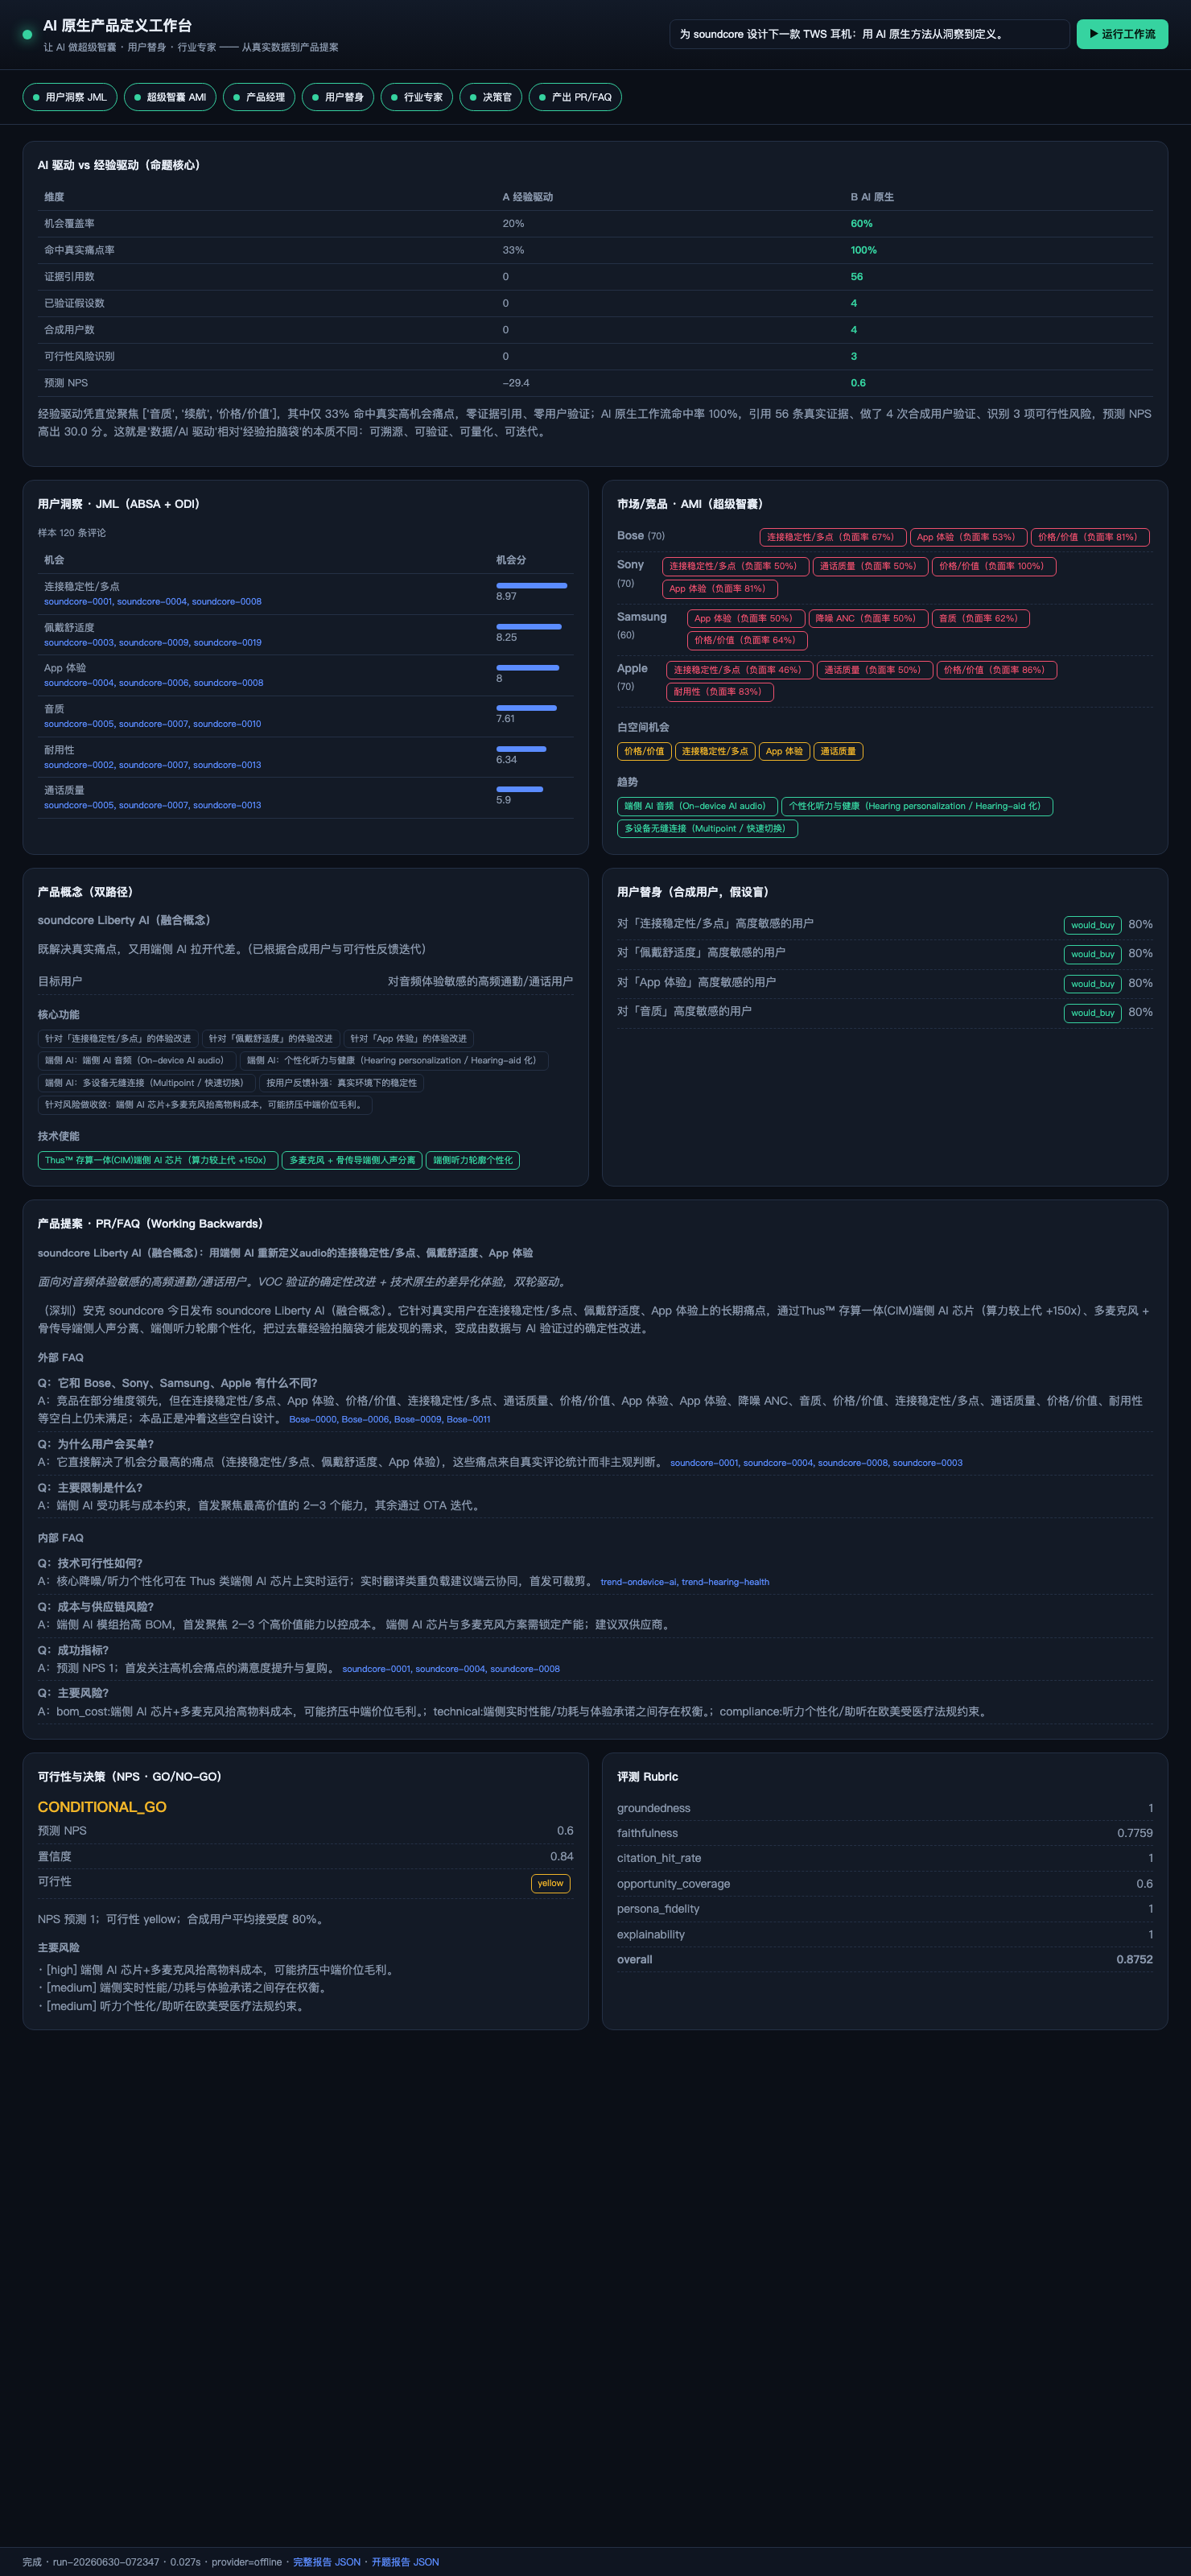
\includegraphics[width=\linewidth]{../figures/demo_full.png}
\captionof{figure}{可视化工作台：每个 Agent 节点实时点亮，并呈现 VOC 机会、竞品白空间、概念、合成用户访谈、PR/FAQ、决策与评测}
\end{center}


\part{工程规范（对标大厂 AIGC）}
\section{为什么规范是"企业级 vs 玩具"的分水岭}

我们对标美团技术团队《用 Agent 评测思路管理 AI Coding——31 万行代码 AI 重构的实践》的核心理念：当 90\% 以上代码由 AI 生成，
\textbf{没有统一规范，系统会加速腐化}。规范在 AI Coding 时代已从"协作建议"升级为"约束 AI 产出、阻止系统继续长新债的基础设施"。
其方法论是\kw{人人对齐 $\rightarrow$ 人机对齐}：先让团队形成统一共识，再把共识固化为 AI 编码时强制加载的约束。

\section{本项目落地的规范}

\begin{itemize}
\item \kw{AI Rule（always-on）}：\texttt{.cursor/rules/} 强制四层架构、Pydantic 数据模型、loguru 日志、完整类型注解、
  工具 \texttt{@tool} 读写分离（WRITE 须两步确认）、\textbf{所有结论强制带 source\_id 引用}。
\item \kw{Skill（渐进式加载）}：\texttt{skills/} 沉淀 VOC 分析、Working Backwards 的可执行 SOP。
\item \kw{Pre-PR 自查}：\texttt{scripts/pre\_pr\_check.py} 在提交前做确定性规范校验（分层、日志、类型、异常），过滤 AI 编码常见低级问题。
\item \kw{跨厂商模型对抗 CR}：\texttt{scripts/cross\_model\_review.py} 用 MiniMax M3 按本仓规范审查代码，对应"高阶模型审低阶 + 不同厂商互审"。
\item \kw{确定性优先}：能用词典/统计/规则得到的结果不交给 LLM，回应"大模型不确定性 vs 企业高确定性"。
\item \kw{异常与降级}：每个外部调用都有 fallback（LLM 不可用 $\rightarrow$ offline；检索为空 $\rightarrow$ 重写重试，上限 3 次），不静默失败。
\end{itemize}

\section{代码风格（与美团一致）}

\begin{lstlisting}[language=Python]
from pydantic import BaseModel, Field   # 必用 Pydantic 数据模型
from loguru import logger               # 必用 loguru，不用 print/logging
from typing import List, Optional       # 完整类型注解

@tool(ToolType.READ)                     # 工具区分读/写；WRITE 须两步确认
def search_evidence(query: str) -> List[Evidence]:
    """检索证据（只读，可并发）。"""
    logger.bind(node="rag").info(f"检索: {query}")
    ...
\end{lstlisting}

\noindent 本项目所有后端模块均通过 \texttt{pre\_pr\_check.py} 校验、\texttt{compileall} 字节编译，并附带冒烟测试
\texttt{backend/tests/test\_smoke.py}（验证端到端跑通且 groundedness/引用命中率达标、AI 组优于经验组）。


\part{部署与运维}
\section{多项目隔离原则}

目标服务器（阿里云 ECS，华南-深圳，Ubuntu 22.04，2 vCPU / 2 GiB）上已运行项目一"小念（xiaonian）"。本项目作为
\textbf{项目二}接入，严格遵循"\textbf{每个项目有且只有：一个代码目录 + 一个 venv + 一个 systemd 服务 +
一个 nginx location + 一个静态目录}"的隔离原则，互不影响、可独立停/改/回滚。

\begin{center}
\begin{tikzpicture}[font=\small,
  box/.style={draw=primary,rounded corners=4pt,fill=primary!6,minimum width=3.0cm,minimum height=0.8cm,align=center,text=ink},
  ext/.style={draw=accent,rounded corners=4pt,fill=accent!8,minimum width=2.6cm,minimum height=0.8cm,align=center,text=ink},
  a/.style={-Latex,thick,color=soft}]
  \node[ext] (user) {公网用户};
  \node[box,right=1.4cm of user] (nginx) {nginx :80\\(唯一入口)};
  \node[box,above right=0.3cm and 1.6cm of nginx] (x) {xiaonian\\:8765};
  \node[box,right=1.6cm of nginx] (a) {anker\\:8766};
  \node[box,below right=0.3cm and 1.6cm of nginx] (hub) {hub 静态\\/var/www/hub};
  \draw[a] (user)--(nginx);
  \draw[a] (nginx)-- node[above,text=soft]{\scriptsize /xiaonian/app/} (x);
  \draw[a] (nginx)-- node[above,text=soft]{\scriptsize /anker/app/} (a);
  \draw[a] (nginx)-- node[below,text=soft]{\scriptsize /} (hub);
\end{tikzpicture}
\captionof{figure}{部署拓扑：nginx 单入口按子路径反代到各自 127.0.0.1 端口；后端不直接暴露公网}
\end{center}

\section{公网路由表}

\begin{table}[h]\centering\small
\renewcommand{\arraystretch}{1.2}
\begin{tabularx}{\linewidth}{p{6.4cm} p{2.6cm} X}
\toprule
\textbf{公网 URL} & \textbf{类型} & \textbf{后端} \\
\midrule
\url{http://47.119.112.225/} & 静态 hub & /var/www/hub \\
\url{http://47.119.112.225/xiaonian/app/} & FastAPI 代理 & 127.0.0.1:8765（项目一，未改动） \\
\url{http://47.119.112.225/anker/} & 静态宣传页 & /var/www/anker \\
\url{http://47.119.112.225/anker/app/} & FastAPI 代理 & 127.0.0.1:8766（本项目） \\
\bottomrule
\end{tabularx}
\caption{部署后公网路由（小念路由完全不受影响）}
\end{table}

\section{部署流程（一键脚本）}

\texttt{scripts/deploy.py}（凭据从环境变量读取，绝不入库）自动完成：本地打包并经 SFTP 上传代码（绕过服务器对 GitHub
的访问不稳定）$\rightarrow$ 创建 venv 并经清华镜像安装依赖 $\rightarrow$ 生成样本数据 $\rightarrow$ 写 \texttt{.env}
（不入库）$\rightarrow$ 创建 \texttt{anker.service} systemd 守护 $\rightarrow$ 落地宣传页 $\rightarrow$ 幂等插入 nginx 路由
$\rightarrow$ 健康检查。子路径反代要点：应用前端统一使用\textbf{相对路径}，nginx \texttt{proxy\_pass} 去前缀后应用即
"根路径"工作，SSE 流式输出需 \texttt{proxy\_buffering off}。

\section{健康检查（部署后实测）}

\begin{lstlisting}[numbers=none]
local-app     200      # 127.0.0.1:8766/api/health
hub           200      # /
xiaonian      200      # /xiaonian/  (项目一未受影响)
anker-landing 200      # /anker/
anker-demo    200      # /anker/app/
/anker/app/api/health  -> {"status":"ok","provider":"offline"}
公网 POST /anker/app/api/run -> decision=CONDITIONAL_GO, overall=0.875,
                                命中真实痛点 A/B = 33% / 100%
\end{lstlisting}

\begin{center}
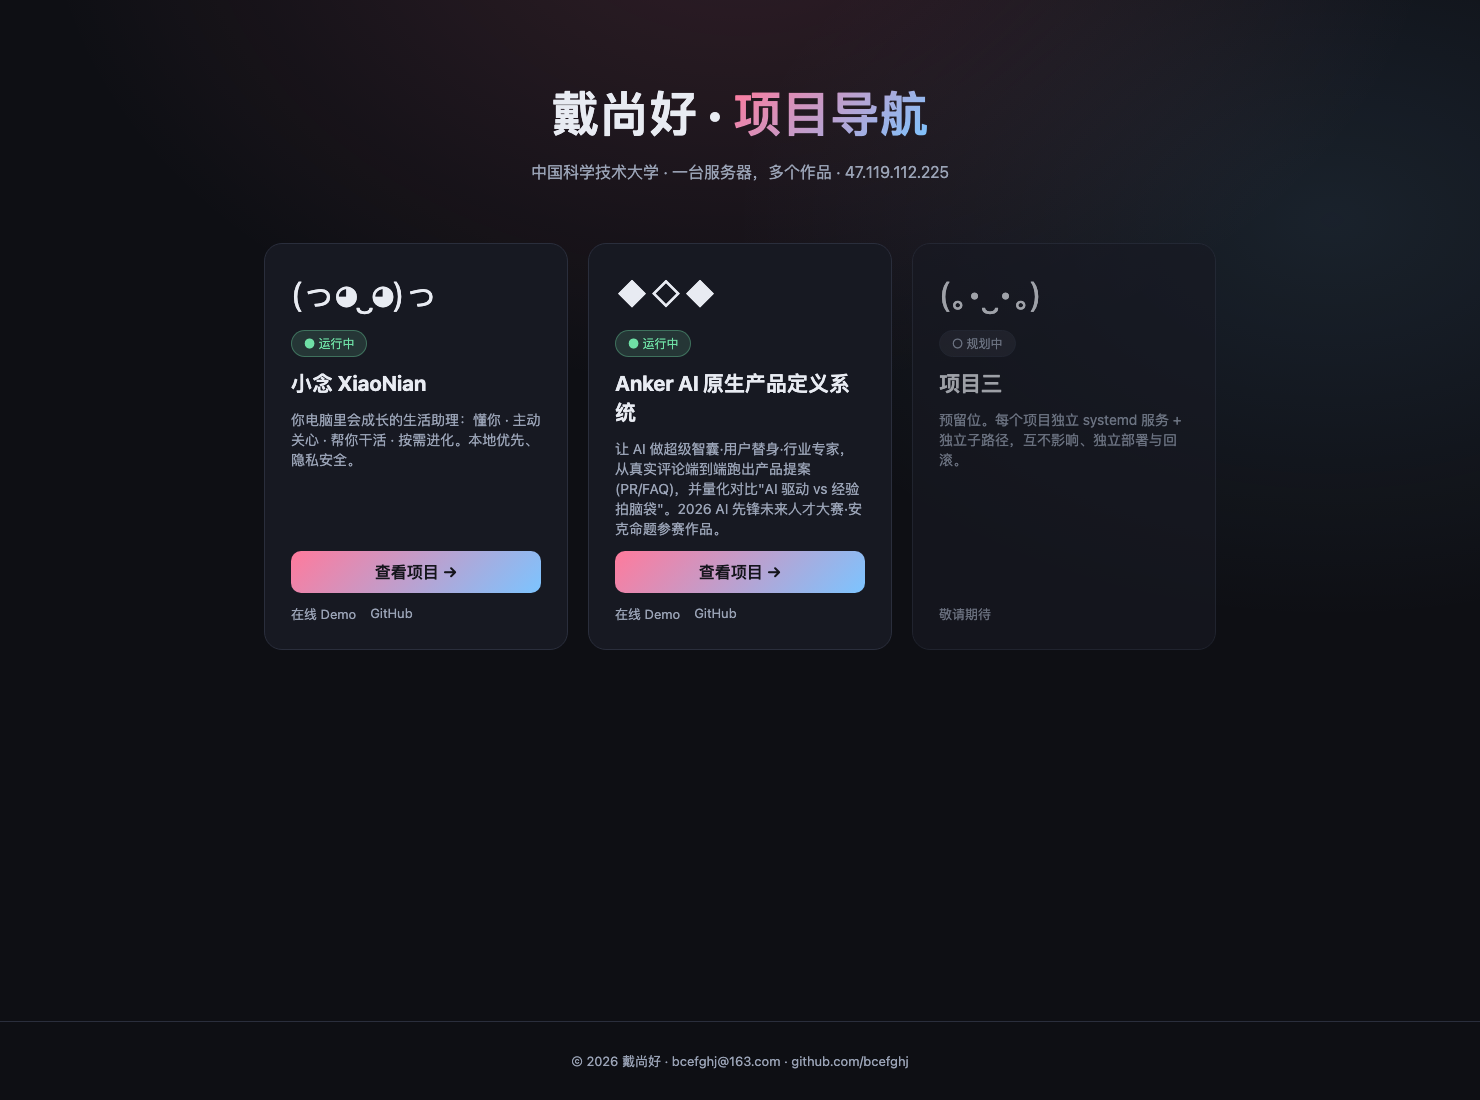
\includegraphics[width=0.92\linewidth]{../figures/hub.png}
\captionof{figure}{项目导航 hub：小念与 Anker 两个作品均"运行中"，互不冲突}
\end{center}

\section{回滚}
停止并禁用 \texttt{anker.service}、注释 nginx 中 anker 的 location、\texttt{nginx -t \&\& systemctl reload nginx} 即可；
小念的服务与路由完全不受影响。


\part{结果展示与链接}
\section{宣传页与在线 Demo}

\begin{center}
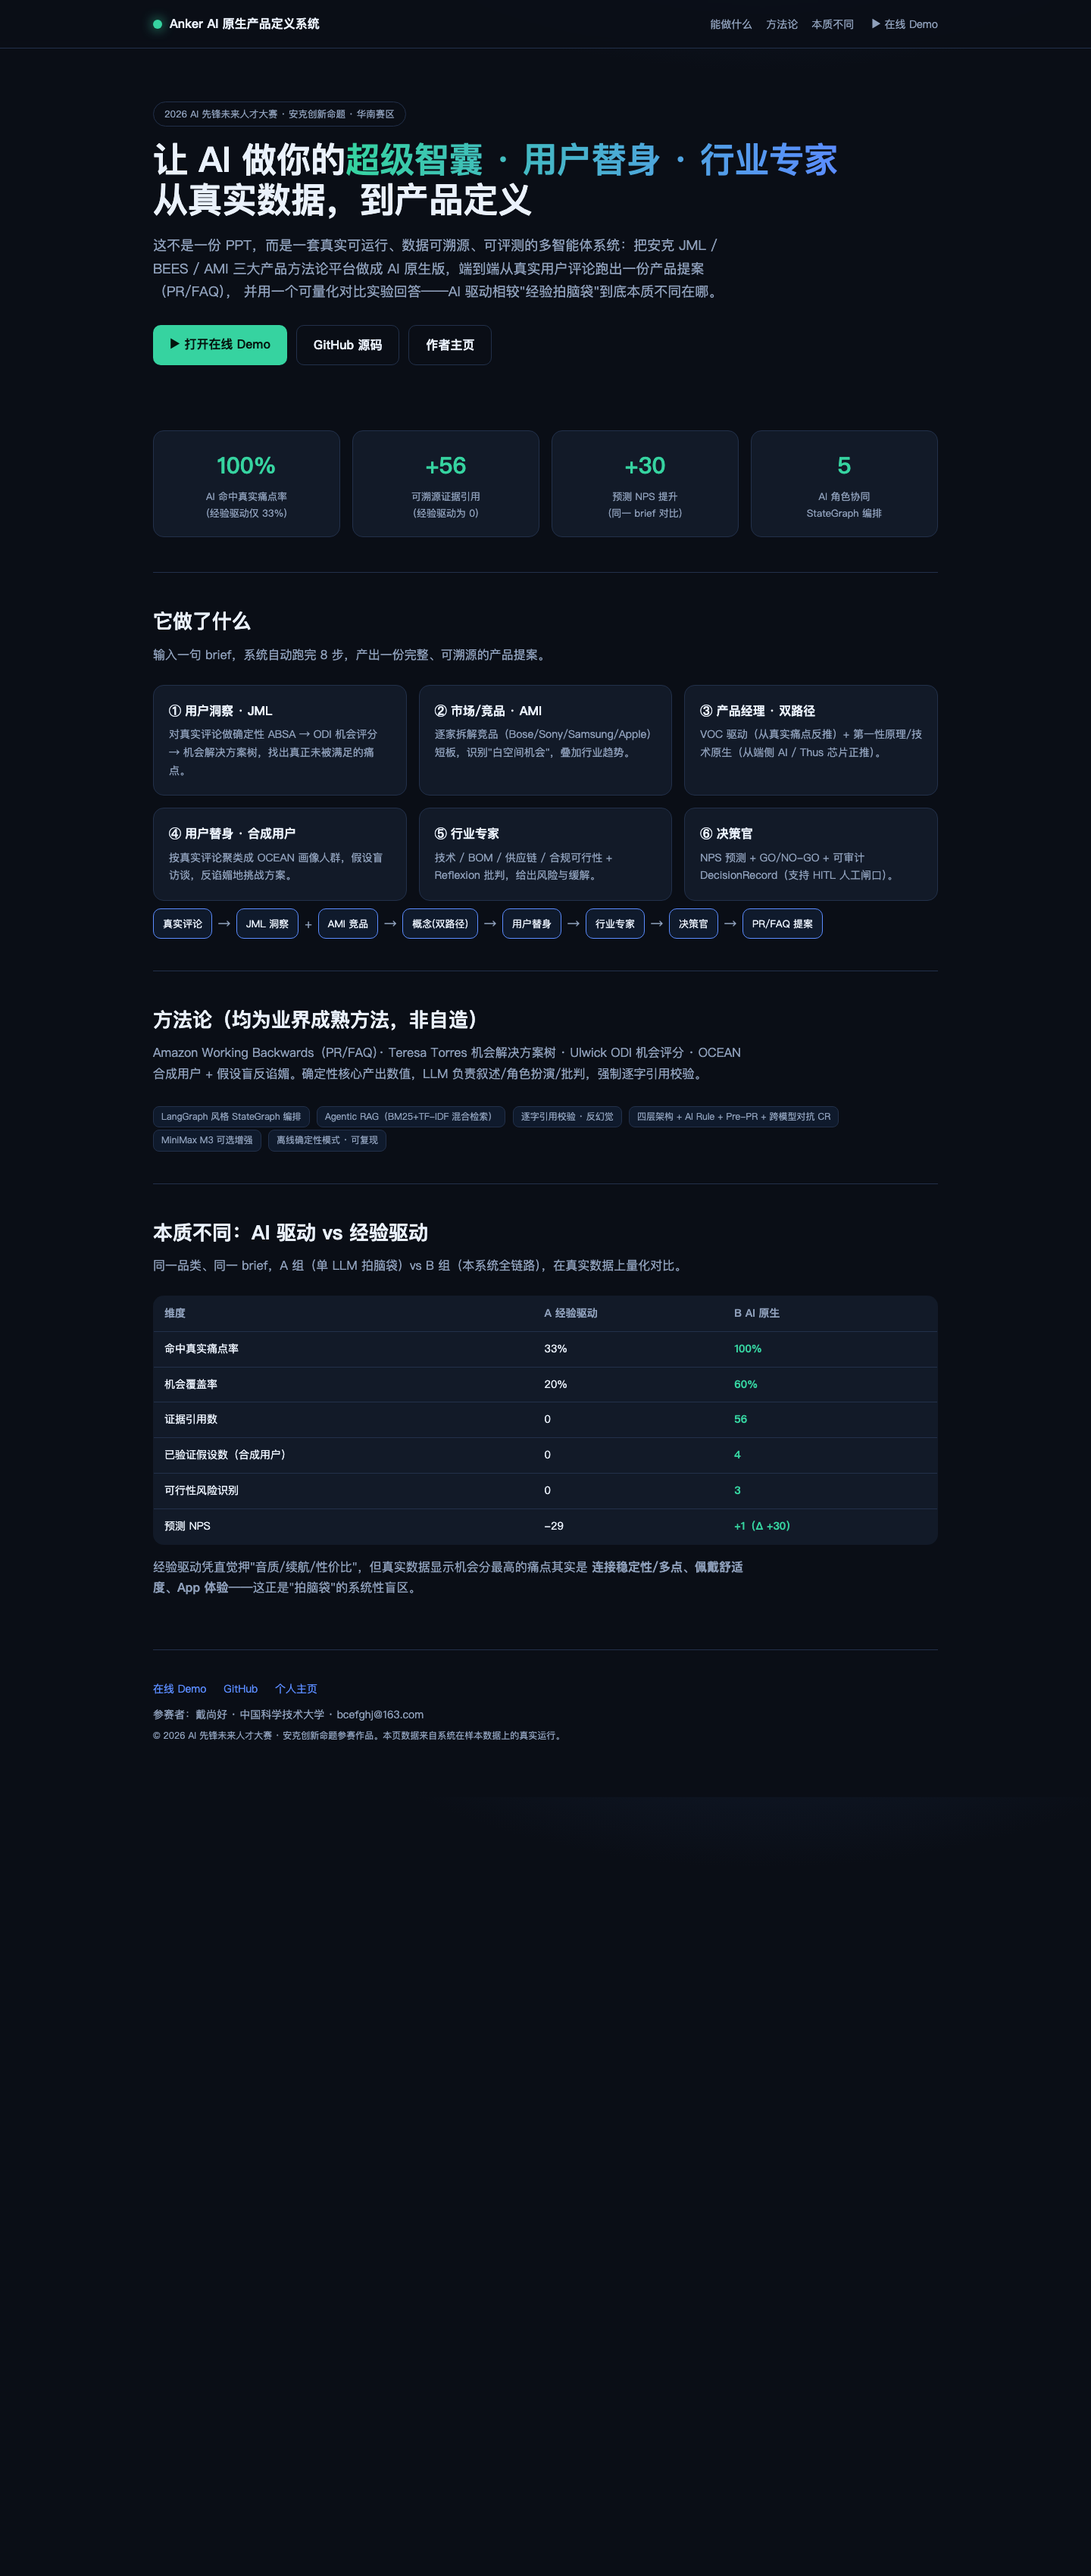
\includegraphics[width=0.86\linewidth]{../figures/landing.png}
\captionof{figure}{项目宣传页（\url{http://47.119.112.225/anker/}）}
\end{center}

\begin{center}
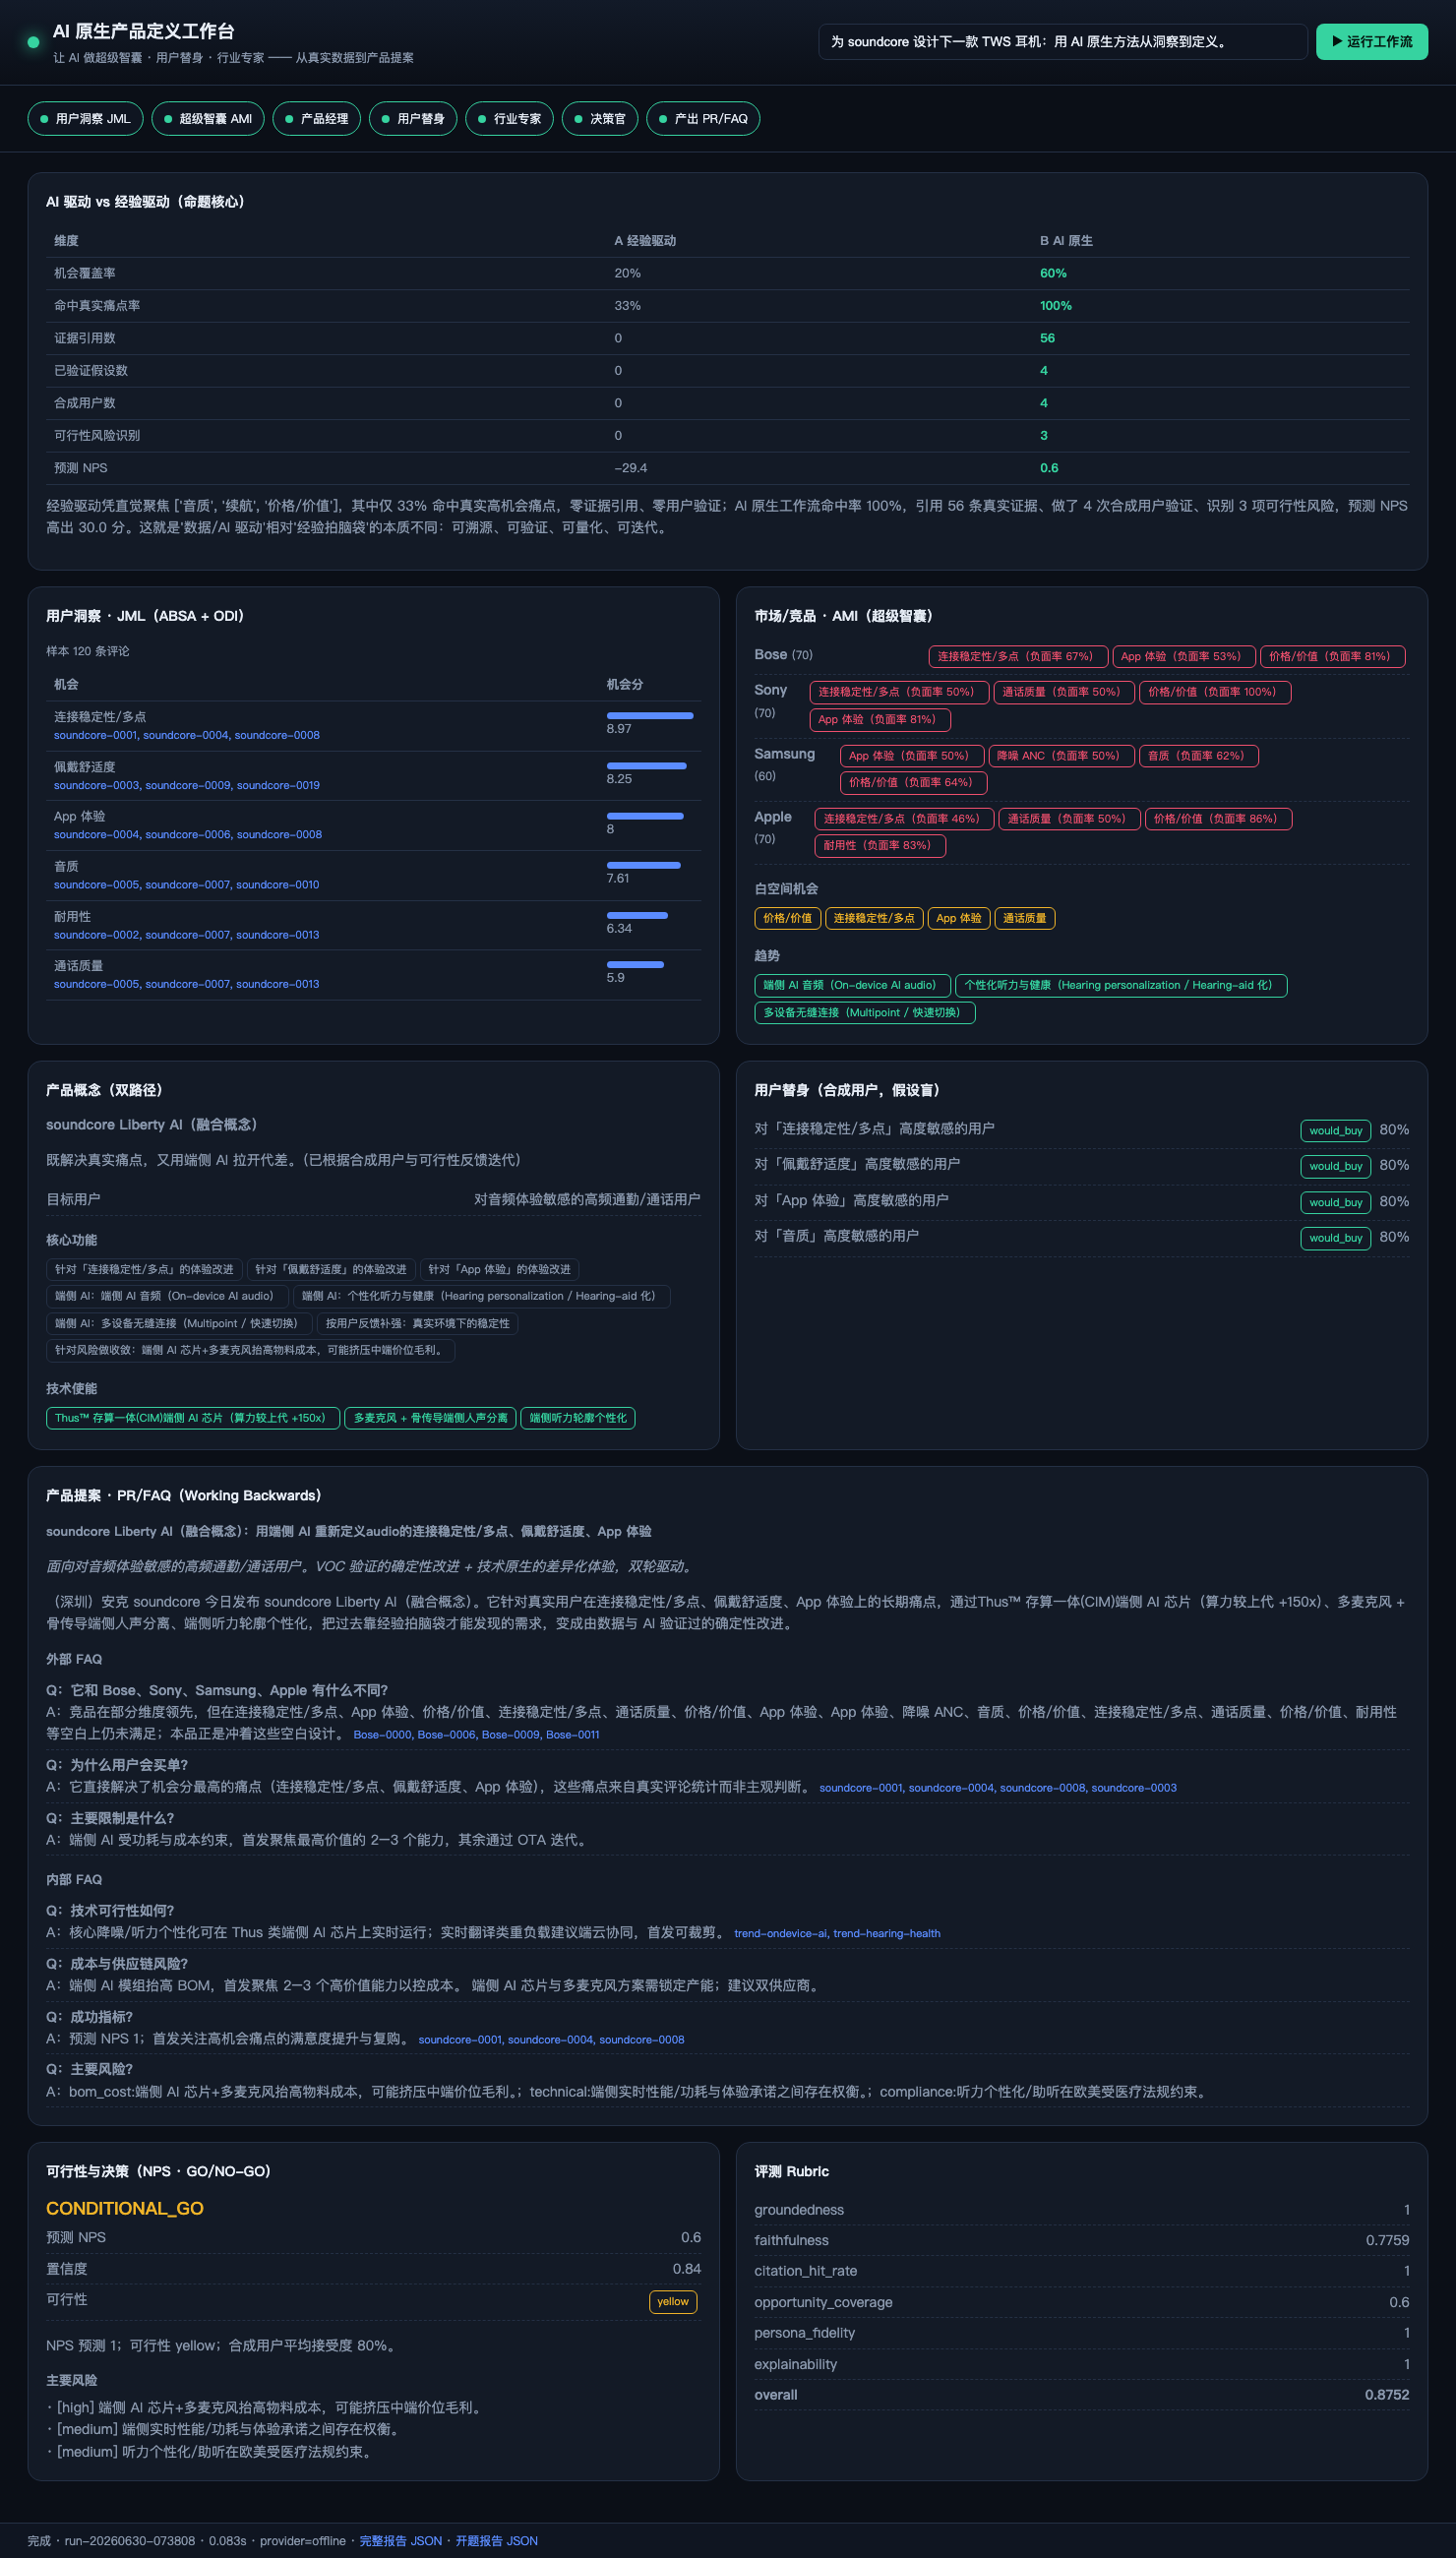
\includegraphics[width=\linewidth]{../figures/deployed_demo.png}
\captionof{figure}{线上 Demo 实跑结果（\url{http://47.119.112.225/anker/app/}）}
\end{center}

\section{链接汇总}
\begin{itemize}
\item 在线 Demo：\url{http://47.119.112.225/anker/app/}
\item 项目宣传页：\url{http://47.119.112.225/anker/}
\item 项目导航 Hub：\url{http://47.119.112.225/}
\item GitHub 源码：\url{https://github.com/bcefghj/anker-ai-product-studio}
\item 个人主页：\url{https://bcefghj.github.io}
\end{itemize}

\section{复现指南}
\begin{lstlisting}[language=bash,numbers=none]
# 1) 离线确定性模式（零网络、可复现）
pip install -r requirements.txt
python3 data/make_sample.py
PYTHONPATH=backend python3 -m anker_studio.starter.cli run
# 2) 可视化工作台
PYTHONPATH=backend python3 -m uvicorn anker_studio.starter.api:app --port 8000
# 3) 接入 MiniMax M3：在 .env 设 MINIMAX_API_KEY 并 ANKER_LLM_PROVIDER=minimax
# 4) 用真实 Amazon 评论：python3 -m anker_studio.infrastructure.data.amazon_reviews
\end{lstlisting}

\section{局限与未来工作}
\begin{itemize}
\item 合成用户与离线评分是"发现 + 排序"工具，不替代真实用户终验（与 NN/g 结论一致）；建议作为 AI 原生方法前置问题空间、把研究预算花在刀刃上。
\item 线上 Demo 默认 offline 确定性模式以保证稳定与零成本；接入 MiniMax M3 可增强叙述质量与多模态。
\item 可对接安克 AIME 平台，把本 SOP 沉淀为内部新 Agent 能力；并扩展到充电、eufy 等品类（仅需更换数据配置与 aspect 词典）。
\item 可引入更强的 ABSA 模型（BERT 类）与真实 A/B 实验闭环，进一步提升机会识别与 NPS 预测精度。
\end{itemize}

\section{结语}
本作品用一套真实可运行、可溯源、可评测的系统回答了命题：AI 原生的产品定义，不是"让 AI 帮你更快拍脑袋"，而是把产品判断
从个人经验升级为可复制的系统能力——这正是安克"用 AI 重新定义怎么想出一个好产品"的方向。


% ====================================================================
\appendix
\part{附录}
\section*{附录说明}
\addcontentsline{toc}{section}{附录说明}

以下为本项目\textbf{全部核心源码}的逐文件清单（真实代码，非节选），按四层架构与逻辑顺序组织，便于评委审阅工程实现。
代码总量约 4{,}500 行（后端 Python 约 3{,}600 行 + 前端/脚本/配置）。每个文件标注其相对路径与行数。

\vspace{0.4cm}
\noindent 阅读建议：
\begin{itemize}
\item 先看 \texttt{common/models.py}（贯穿全系统的 Pydantic 领域模型）与 \texttt{common/citations.py}（反幻觉引用校验）。
\item 再看 \texttt{infrastructure/nlp/absa.py}（确定性 ABSA 核心）与 \texttt{application/methodology/odi.py}（机会量化）。
\item 然后看五个 Agent 与 \texttt{application/graph/}（StateGraph 编排引擎）。
\item 最后看 \texttt{application/evaluation/}（Rubric 与 AI/经验对比）与部署脚本 \texttt{scripts/deploy.py}。
\end{itemize}
\vspace{0.3cm}

% 自动生成：源码附录。请用 gen_appendix.py 重新生成。

\section{Common 层（领域模型 / 配置 / 工具 / 引用校验）}
\subsection*{\texttt{backend/anker\_studio/common/models.py} \hfill \normalfont\small (299 行)}
\lstinputlisting[language=Python]{../../backend/anker_studio/common/models.py}

\subsection*{\texttt{backend/anker\_studio/common/config.py} \hfill \normalfont\small (68 行)}
\lstinputlisting[language=Python]{../../backend/anker_studio/common/config.py}

\subsection*{\texttt{backend/anker\_studio/common/logging.py} \hfill \normalfont\small (31 行)}
\lstinputlisting[language=Python]{../../backend/anker_studio/common/logging.py}

\subsection*{\texttt{backend/anker\_studio/common/tools.py} \hfill \normalfont\small (58 行)}
\lstinputlisting[language=Python]{../../backend/anker_studio/common/tools.py}

\subsection*{\texttt{backend/anker\_studio/common/citations.py} \hfill \normalfont\small (117 行)}
\lstinputlisting[language=Python]{../../backend/anker_studio/common/citations.py}

\section{Infrastructure 层（LLM 网关 / 数据 / RAG / NLP / 媒体 / 观测）}
\subsection*{\texttt{backend/anker\_studio/infrastructure/llm/gateway.py} \hfill \normalfont\small (107 行)}
\lstinputlisting[language=Python]{../../backend/anker_studio/infrastructure/llm/gateway.py}

\subsection*{\texttt{backend/anker\_studio/infrastructure/llm/minimax.py} \hfill \normalfont\small (62 行)}
\lstinputlisting[language=Python]{../../backend/anker_studio/infrastructure/llm/minimax.py}

\subsection*{\texttt{backend/anker\_studio/infrastructure/data/loader.py} \hfill \normalfont\small (113 行)}
\lstinputlisting[language=Python]{../../backend/anker_studio/infrastructure/data/loader.py}

\subsection*{\texttt{backend/anker\_studio/infrastructure/data/amazon\_reviews.py} \hfill \normalfont\small (122 行)}
\lstinputlisting[language=Python]{../../backend/anker_studio/infrastructure/data/amazon_reviews.py}

\subsection*{\texttt{backend/anker\_studio/infrastructure/data/connectors.py} \hfill \normalfont\small (71 行)}
\lstinputlisting[language=Python]{../../backend/anker_studio/infrastructure/data/connectors.py}

\subsection*{\texttt{backend/anker\_studio/infrastructure/nlp/lexicons.py} \hfill \normalfont\small (55 行)}
\lstinputlisting[language=Python]{../../backend/anker_studio/infrastructure/nlp/lexicons.py}

\subsection*{\texttt{backend/anker\_studio/infrastructure/nlp/absa.py} \hfill \normalfont\small (108 行)}
\lstinputlisting[language=Python]{../../backend/anker_studio/infrastructure/nlp/absa.py}

\subsection*{\texttt{backend/anker\_studio/infrastructure/rag/retrieval.py} \hfill \normalfont\small (138 行)}
\lstinputlisting[language=Python]{../../backend/anker_studio/infrastructure/rag/retrieval.py}

\subsection*{\texttt{backend/anker\_studio/infrastructure/assets/media.py} \hfill \normalfont\small (64 行)}
\lstinputlisting[language=Python]{../../backend/anker_studio/infrastructure/assets/media.py}

\subsection*{\texttt{backend/anker\_studio/infrastructure/observability/trace.py} \hfill \normalfont\small (68 行)}
\lstinputlisting[language=Python]{../../backend/anker_studio/infrastructure/observability/trace.py}

\section{Application 层 · 方法论（ODI / OST / Working Backwards）}
\subsection*{\texttt{backend/anker\_studio/application/methodology/odi.py} \hfill \normalfont\small (78 行)}
\lstinputlisting[language=Python]{../../backend/anker_studio/application/methodology/odi.py}

\subsection*{\texttt{backend/anker\_studio/application/methodology/ost.py} \hfill \normalfont\small (85 行)}
\lstinputlisting[language=Python]{../../backend/anker_studio/application/methodology/ost.py}

\subsection*{\texttt{backend/anker\_studio/application/methodology/working\_backwards.py} \hfill \normalfont\small (107 行)}
\lstinputlisting[language=Python]{../../backend/anker_studio/application/methodology/working_backwards.py}

\section{Application 层 · 安克三平台（JML / AMI / BEES）}
\subsection*{\texttt{backend/anker\_studio/application/platforms/jml.py} \hfill \normalfont\small (33 行)}
\lstinputlisting[language=Python]{../../backend/anker_studio/application/platforms/jml.py}

\subsection*{\texttt{backend/anker\_studio/application/platforms/ami.py} \hfill \normalfont\small (73 行)}
\lstinputlisting[language=Python]{../../backend/anker_studio/application/platforms/ami.py}

\subsection*{\texttt{backend/anker\_studio/application/platforms/bees.py} \hfill \normalfont\small (113 行)}
\lstinputlisting[language=Python]{../../backend/anker_studio/application/platforms/bees.py}

\section{Application 层 · 五个 Agent}
\subsection*{\texttt{backend/anker\_studio/application/agents/base.py} \hfill \normalfont\small (39 行)}
\lstinputlisting[language=Python]{../../backend/anker_studio/application/agents/base.py}

\subsection*{\texttt{backend/anker\_studio/application/agents/super\_think\_tank.py} \hfill \normalfont\small (56 行)}
\lstinputlisting[language=Python]{../../backend/anker_studio/application/agents/super_think_tank.py}

\subsection*{\texttt{backend/anker\_studio/application/agents/product\_manager.py} \hfill \normalfont\small (132 行)}
\lstinputlisting[language=Python]{../../backend/anker_studio/application/agents/product_manager.py}

\subsection*{\texttt{backend/anker\_studio/application/agents/user\_proxy.py} \hfill \normalfont\small (138 行)}
\lstinputlisting[language=Python]{../../backend/anker_studio/application/agents/user_proxy.py}

\subsection*{\texttt{backend/anker\_studio/application/agents/industry\_expert.py} \hfill \normalfont\small (88 行)}
\lstinputlisting[language=Python]{../../backend/anker_studio/application/agents/industry_expert.py}

\subsection*{\texttt{backend/anker\_studio/application/agents/decision\_officer.py} \hfill \normalfont\small (80 行)}
\lstinputlisting[language=Python]{../../backend/anker_studio/application/agents/decision_officer.py}

\section{Application 层 · 编排 / 评测 / 对照 / 报告}
\subsection*{\texttt{backend/anker\_studio/application/graph/state.py} \hfill \normalfont\small (74 行)}
\lstinputlisting[language=Python]{../../backend/anker_studio/application/graph/state.py}

\subsection*{\texttt{backend/anker\_studio/application/graph/engine.py} \hfill \normalfont\small (114 行)}
\lstinputlisting[language=Python]{../../backend/anker_studio/application/graph/engine.py}

\subsection*{\texttt{backend/anker\_studio/application/graph/checkpoint.py} \hfill \normalfont\small (34 行)}
\lstinputlisting[language=Python]{../../backend/anker_studio/application/graph/checkpoint.py}

\subsection*{\texttt{backend/anker\_studio/application/graph/pipeline.py} \hfill \normalfont\small (110 行)}
\lstinputlisting[language=Python]{../../backend/anker_studio/application/graph/pipeline.py}

\subsection*{\texttt{backend/anker\_studio/application/baseline/experience\_driven.py} \hfill \normalfont\small (50 行)}
\lstinputlisting[language=Python]{../../backend/anker_studio/application/baseline/experience_driven.py}

\subsection*{\texttt{backend/anker\_studio/application/evaluation/rubric.py} \hfill \normalfont\small (67 行)}
\lstinputlisting[language=Python]{../../backend/anker_studio/application/evaluation/rubric.py}

\subsection*{\texttt{backend/anker\_studio/application/evaluation/comparison.py} \hfill \normalfont\small (91 行)}
\lstinputlisting[language=Python]{../../backend/anker_studio/application/evaluation/comparison.py}

\subsection*{\texttt{backend/anker\_studio/application/runner.py} \hfill \normalfont\small (114 行)}
\lstinputlisting[language=Python]{../../backend/anker_studio/application/runner.py}

\subsection*{\texttt{backend/anker\_studio/application/reporting.py} \hfill \normalfont\small (232 行)}
\lstinputlisting[language=Python]{../../backend/anker_studio/application/reporting.py}

\section{Starter 层（CLI / FastAPI）与入口}
\subsection*{\texttt{backend/anker\_studio/starter/cli.py} \hfill \normalfont\small (81 行)}
\lstinputlisting[language=Python]{../../backend/anker_studio/starter/cli.py}

\subsection*{\texttt{backend/anker\_studio/starter/api.py} \hfill \normalfont\small (103 行)}
\lstinputlisting[language=Python]{../../backend/anker_studio/starter/api.py}

\subsection*{\texttt{run.py} \hfill \normalfont\small (27 行)}
\lstinputlisting[language=Python]{../../run.py}

\section{前端工作台（零依赖可视化）}
\subsection*{\texttt{frontend/index.html} \hfill \normalfont\small (77 行)}
\lstinputlisting[language=HTML]{../../frontend/index.html}

\subsection*{\texttt{frontend/app.js} \hfill \normalfont\small (168 行)}
\lstinputlisting[]{../../frontend/app.js}

\subsection*{\texttt{frontend/styles.css} \hfill \normalfont\small (75 行)}
\lstinputlisting[]{../../frontend/styles.css}

\section{宣传 Landing 页}
\subsection*{\texttt{web/landing/index.html} \hfill \normalfont\small (152 行)}
\lstinputlisting[language=HTML]{../../web/landing/index.html}

\section{工程规范与运维脚本}
\subsection*{\texttt{.cursor/rules/00-engineering-baseline.mdc} \hfill \normalfont\small (47 行)}
\lstinputlisting[]{../../.cursor/rules/00-engineering-baseline.mdc}

\subsection*{\texttt{.cursor/rules/10-agent-conventions.mdc} \hfill \normalfont\small (29 行)}
\lstinputlisting[]{../../.cursor/rules/10-agent-conventions.mdc}

\subsection*{\texttt{scripts/pre\_pr\_check.py} \hfill \normalfont\small (79 行)}
\lstinputlisting[language=Python]{../../scripts/pre_pr_check.py}

\subsection*{\texttt{scripts/cross\_model\_review.py} \hfill \normalfont\small (78 行)}
\lstinputlisting[language=Python]{../../scripts/cross_model_review.py}

\subsection*{\texttt{scripts/deploy.py} \hfill \normalfont\small (188 行)}
\lstinputlisting[language=Python]{../../scripts/deploy.py}

\subsection*{\texttt{scripts/server\_exec.py} \hfill \normalfont\small (35 行)}
\lstinputlisting[language=Python]{../../scripts/server_exec.py}

\subsection*{\texttt{scripts/update\_hub.py} \hfill \normalfont\small (60 行)}
\lstinputlisting[language=Python]{../../scripts/update_hub.py}

\subsection*{\texttt{data/make\_sample.py} \hfill \normalfont\small (133 行)}
\lstinputlisting[language=Python]{../../data/make_sample.py}

\subsection*{\texttt{backend/tests/test\_smoke.py} \hfill \normalfont\small (45 行)}
\lstinputlisting[language=Python]{../../backend/tests/test_smoke.py}


\end{document}
